\section{Arithmetic Operations}



\begin{definition}{Basic Arithmetic Instructions}\\
Core arithmetic operations:
\begin{itemize}
  \item \textbf{ADD/ADDS}: Addition ($A + B$)
  \item \textbf{ADCS}: Addition with Carry ($A + B + c$)
  \item \textbf{ADR}: Address to Register ($PC + A$)
  \item \textbf{SUB/SUBS}: Subtraction ($A - B$)
  \item \textbf{SBCS}: Subtraction with carry/borrow ($A - B - !c$)
  \item \textbf{RSBS}: Reverse Subtract ($-1 \cdot A$)
  \item \textbf{MULS}: Multiplication ($A \cdot B$)
\end{itemize}
\end{definition}

\begin{formula}{Addition Operations}
Addition instructions and their uses:
\begin{itemize}
  \item \textbf{ADDS Rd, Rn, Rm} $\rightarrow$ Rd = Rn + Rm
  \begin{itemize}
    \item Updates flags, only low registers
  \end{itemize}
  \item \textbf{ADD Rd, Rm} $\rightarrow$ Rd = Rd + Rm
  \begin{itemize}
    \item No flag updates, can use high registers
  \end{itemize}
  \item \textbf{ADDS Rd, \#imm} $\rightarrow$ Rd = Rd + immediate
  \begin{itemize}
    \item 8-bit immediate value only
  \end{itemize}
\end{itemize}
\begin{lstlisting}[language=armasm, style=basesmol]
; Different ADD variants
ADDS    R1, R2, R3      ; R1 = R2 + R3, update flags
ADD     R8, R9          ; R8 = R8 + R9, no flags
ADDS    R1, #255        ; R1 = R1 + 255, update flags
\end{lstlisting}
\end{formula}

\begin{formula}{Subtraction Operations}
Subtraction instructions and their uses:
\begin{itemize}
  \item \textbf{SUBS Rd, Rn, Rm} $\rightarrow$ Rd = Rn - Rm
    \begin{itemize}
      \item Updates flags, only low registers
    \end{itemize}
  \item \textbf{SUBS Rd, \#imm} $\rightarrow$ Rd = Rd - immediate
    \begin{itemize}
      \item 8-bit immediate value
    \end{itemize}
  \item \textbf{RSBS Rd, Rn, \#0} $\rightarrow$ Rd = -Rn (2's complement)
    \begin{itemize}
      \item Special case for negation
    \end{itemize}
\end{itemize}
\begin{lstlisting}[language=armasm, style=basesmol]
; Different SUB variants
SUBS    R1, R2, R3      ; R1 = R2 - R3
SUBS    R1, #100        ; R1 = R1 - 100
RSBS    R1, R2, #0      ; R1 = -R2
\end{lstlisting}
\end{formula}

\begin{example2}{Multiplication}
\begin{lstlisting}[language=armasm, style=basesmol]
; Basic multiplication
MULS    R0, R1, R0      ; R0 = R1 * R0
; Multiply by constant using shifts
LSLS    R0, R0, #2      ; R0 = R0 * 4
; Multiply by 10 (8 + 2)
LSLS    R1, R0, #3      ; R1 = R0 * 8
LSLS    R2, R0, #1      ; R2 = R0 * 2
ADDS    R0, R1, R2      ; R0 = R0 * 10
\end{lstlisting}
\end{example2}

\begin{KR}{Arithmetic Operations}
Steps for arithmetic operations:
\begin{enumerate}
  \item Determine if operation is signed or unsigned
  \item Choose appropriate instruction (with or without 'S')
  \begin{itemize}
    \item Use ADDS/SUBS for low registers with flags
    \item Use ADD/SUB for high registers
    \item For immediate values > 8-bit, load to register first
  \end{itemize}
  \item Consider potential carry/overflow conditions
  \item For multi-word operations: see KR \textcolor{pink}{\textbf{Multi-Word Operations}}
  \item Check relevant flags after operation: see \textcolor{darkturquoise}{\textbf{Processor Status Flags}}
\end{enumerate}
\end{KR}

\subsubsection{Signed vs. Unsigned Arithmetic}

\begin{definition}{Two's Complement}
For negative numbers:
\begin{itemize}
  \item Two's complement: $A = !A + 1$ (Invert all bits and add 1 to result)
  \item Used for representing signed numbers
  \item Enables using same hardware for addition and subtraction
\end{itemize}
\end{definition}

\begin{concept}{Carry and Overflow}\\
\textbf{Unsigned Operations:}
\begin{itemize}
  \item Addition: C = 1 indicates carry (result too large for available bits)
  \item Subtraction: C = 0 indicates borrow (result negative)
\end{itemize}

\textbf{Signed Operations:}
\begin{itemize}
  \item Addition: V = 1 if overflow with operands of same sign
  \item Subtraction: V = 1 if overflow with operands of opposite signs
\end{itemize}
\end{concept}

\begin{concept}{Number Circles and Two's Complement}

\begin{minipage}{0.45\linewidth}
  Understanding arithmetic\\ wrap-around:
\begin{itemize}
  \item Fixed number of bits creates \\circular number space
  \item Addition moves clockwise \\on number circle
  \item Subtraction moves \\counter-clockwise
\end{itemize}
\end{minipage}
\begin{minipage}{0.5\linewidth}
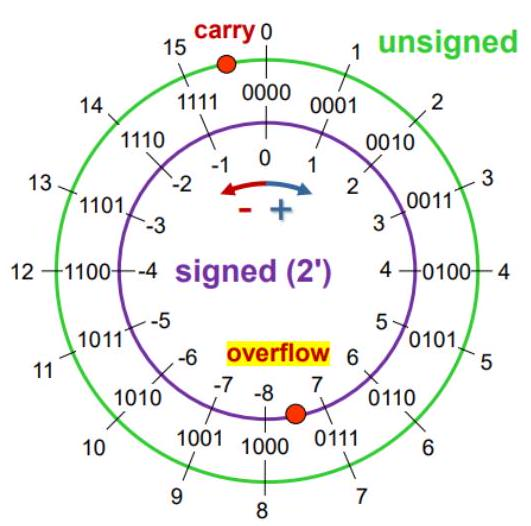
\includegraphics[width=\linewidth]{images/2024_12_29_79e6b22f503fb7b4f718g-04(2)}
\end{minipage}
\vspace{2mm}\\
\begin{minipage}[t]{0.4\linewidth}
Addition: C = 1 $\rightarrow$ Carry

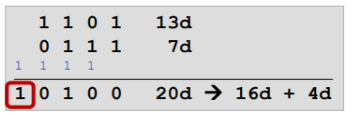
\includegraphics[width=\linewidth]{images/addcarry.png}
\end{minipage}
\begin{minipage}[t]{0.55\linewidth}
Subtraction: C = 0 $\rightarrow$ Borrow

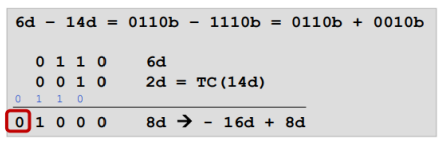
\includegraphics[width=\linewidth]{images/subborrow.png}
\end{minipage}
\end{concept}

\begin{example2}{Integer Ranges by Word Size}\\
\textbf{8-bit integers:}
\begin{itemize}
  \item Unsigned: 0 to 255 (0x00 to 0xFF)
  \item Signed: -128 to 127 (0x80 to 0x7F)
\end{itemize}

\textbf{16-bit integers:}
\begin{itemize}
  \item Unsigned: 0 to 65,535 (0x0000 to 0xFFFF)
  \item Signed: -32,768 to 32,767 (0x8000 to 0x7FFF)
\end{itemize}

\textbf{32-bit integers:}
\begin{itemize}
  \item Unsigned: 0 to 4,294,967,295 (0x00000000 to 0xFFFFFFFF)
  \item Signed: -2,147,483,648 to 2,147,483,647 (0x80000000 to 0x7FFFFFFF)
\end{itemize}
\end{example2}

\begin{KR}{Memory Operations for Arithmetic Operation Patterns}
\begin{lstlisting}[language=armasm, style=basesmol]
; Pattern for modifying memory value
LDR     Rx, =variable     ; Get address
LDR     Ry, [Rx]         ; Load value
; Perform operation
STR     Ry, [Rx]         ; Store result
; For 16-bit values
LDRH/STRH                ; Use half-word instructions
; For 8-bit values
LDRB/STRB                ; Use byte instructions
\end{lstlisting}
\end{KR}

\subsubsection{Flag Usage and Overflow Detection}

\begin{concept}{Processor Status Flags}\\
APSR (Application Program Status Register) contains important flags affected by arithmetic operations:
\begin{itemize}
  \item \textbf{N} (Negative): Set when result's MSB = 1, used for signed operations
  \item \textbf{Z} (Zero): Set when result = 0, used for both signed/unsigned
  \item \textbf{C} (Carry): Set when unsigned overflow occurs
  \item \textbf{V} (Overflow): Set when signed overflow occurs
\end{itemize}

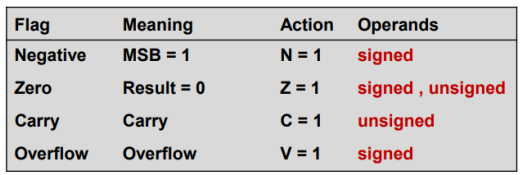
\includegraphics[width=\linewidth]{images/flags-arithmetic.png}

Instructions ending with 'S' modify these flags:
\begin{itemize}
  \item ADDS, SUBS, MOVS, LSLS
\end{itemize}
\end{concept}

\begin{KR}{Overflow Detection}\\
Steps to detect overflow in arithmetic operations:

1. For unsigned arithmetic (using C flag):
\begin{itemize}
  \item Addition: Check C flag (C=1 means overflow)
  \item Subtraction: Check C flag (C=0 means underflow)
\end{itemize}

2. For signed arithmetic (using V flag):
\begin{itemize}
  \item Addition: Check V flag for same-sign operands
  \item Subtraction: Check V flag for opposite-sign operands
\end{itemize}

Example:
\begin{lstlisting}[language=armasm, style=basesmol]
    ; Unsigned overflow detection
    ADDS    R0, R1          ; Perform addition
    BCS     overflow        ; Branch if carry set
    
    ; Signed overflow detection
    ADDS    R0, R1          ; Perform addition
    BVS     overflow        ; Branch if overflow set
\end{lstlisting}
\end{KR}

\begin{example2}{Flag Usage}
Examples of flag behavior:
\begin{lstlisting}[language=armasm, style=basesmol]
; Zero flag example
MOVS    R0, #5
SUBS    R0, #5          ; Z=1 (result is zero)

; Negative flag example
MOVS    R0, #1
SUBS    R0, #2          ; N=1 (result is negative)

; Carry flag example
MOVS    R0, #0xFF
ADDS    R0, #1          ; C=1 (unsigned overflow)

; Overflow flag example
MOVS    R0, #0x7F       ; Max positive 8-bit
ADDS    R0, #1          ; V=1 (signed overflow)
\end{lstlisting}
\end{example2}

\columnbreak

\subsubsection{Examples for basic arithmetic operations}

\begin{example2}{Basic Arithmetic Operations}\\
Given variables in data section:
\begin{lstlisting}[language=armasm, style=basesmol]
    AREA    progData, DATA, READWRITE
Zahl1   DCD     0      ; 32 bit
Zahl2   DCD     0      ; 32 bit 
Zahl3   DCW     0      ; 16 bit
Zahl4   DCW     0      ; 16 bit
Zahl5   DCB     0      ; 8 bit
Zahl6   DCB     0      ; 8 bit
\end{lstlisting}

Basic register operations:

\begin{minipage}{0.4\linewidth}
\begin{lstlisting}[language=armasm, style=basesmol]
; R0 = R1 + R2
ADDS    R0, R1, R2

; R0 = R1 + R2 + R3
ADDS    R0, R1, R2
ADDS    R0, R0, R3

; R8 = R8 + 1
MOVS    R0, #1
ADD     R8, R8, R0

; R8 = -R8
MOV     R7, R8
RSBS    R7, #0
MOV     R8, R7
\end{lstlisting}
\end{minipage}
\hspace{4mm}
\begin{minipage}{0.5\linewidth}
\begin{lstlisting}[language=armasm, style=basesmol]
; R1 = R2 + 200
MOVS    R1, #200
ADD     R1, R1, R2 
; Not ADDS R1,R2,#200 
; invalid, rd = rn    

; R10 = R8 - R7
MOV     R0, R8
SUBS    R0, R0, R7
MOV     R10, R0
\end{lstlisting}
\end{minipage}
\vspace{2mm}\\
Operations involving memory variables:
\begin{lstlisting}[language=armasm, style=basesmol]
; Zahl1 = Zahl1 - 1
LDR     R1, =Zahl1     ; Get address
LDR     R0, [R1]       ; Load value
SUBS    R0, #1         ; Decrement
STR     R0, [R1]       ; Store back

; Zahl1 = Zahl1 + Zahl2
LDR     R0, =Zahl1
LDR     R1, [R0]       ; Load Zahl1
LDR     R2, =Zahl2
LDR     R3, [R2]       ; Load Zahl2
ADDS    R1, R1, R3     ; Add
STR     R1, [R0]       ; Store result

; Zahl3 = Zahl3 - Zahl4 (unsigned)
LDR     R0, =Zahl3
LDRH    R1, [R0]       ; Load 16-bit
LDR     R2, =Zahl4
LDRH    R3, [R2]
SUBS    R1, R1, R3
STRH    R1, [R0]       ; Store 16-bit

; Zahl1 = R5 * Zahl3 (unsigned)
LDR     R0, =Zahl1
LDR     R1, =Zahl3
LDRH    R2, [R1]
MULS    R2, R5, R2
STR     R2, [R0]
\end{lstlisting}
\end{example2}

\subsubsection{Multi-Word Arithmetic}

\begin{KR}{Multi-Word Arithmetic}
Guidelines for operations on large numbers:

1. Addition sequence:
\begin{lstlisting}[language=armasm, style=basesmol]
    ; 64-bit addition (R1:R0 + R3:R2)
    ADDS    R0, R2          ; Add low words
    ADCS    R1, R3          ; Add high words with carry
\end{lstlisting}

2. Subtraction sequence:
\begin{lstlisting}[language=armasm, style=basesmol]
    ; 64-bit subtraction (R1:R0 - R3:R2)
    SUBS    R0, R2          ; Subtract low words
    SBCS    R1, R3          ; Subtract high words with borrow
\end{lstlisting}

3. Important considerations:
\begin{itemize}
  \item Start with least significant words
  \item Use carry-aware instructions for higher words
  \item Ensure proper register allocation
  \item Track flags through entire operation
\end{itemize}
\end{KR}

\begin{concept}{Multi-Word Operations} Multi-Register Operations\\
Guidelines for multi-word arithmetic:

1. Loading values:
\begin{itemize}
  \item Use LDM to load multiple words efficiently
  \item Consider register allocation carefully for all parts
  \item Keep track of which registers hold which parts
  \item Use temporary registers for high register operations
\end{itemize}

2. Performing operations:
\begin{itemize}
  \item Start with least significant words
  \item Use ADDS/SUBS for first word
  \item Use ADCS/SBCS for subsequent words
  \item Pay attention to carry/borrow propagation
  \item Chain operations for complex expressions
\end{itemize}

3. Storing results:
\begin{itemize}
  \item Use STM for efficient multi-word storage
  \item Maintain proper alignment
  \item Consider word order (endianness)
\end{itemize}

Example 96-bit addition:
\begin{lstlisting}[language=armasm, style=basesmol]
    ; Load values
    LDR     R0, =value1
    LDM     R0!, {R1-R3}     ; First number
    LDR     R0, =value2
    LDM     R0!, {R4-R6}     ; Second number
    
    ; Add with carry
    ADDS    R1, R1, R4       ; Low word
    ADCS    R2, R2, R5       ; Middle word
    ADCS    R3, R3, R6       ; High word
    
    ; Store result
    LDR     R0, =result
    STM     R0!, {R1-R3}
\end{lstlisting}
\end{concept}

\begin{remark}
Important considerations:
\begin{itemize}
  \item Always handle carry/borrow for multi-word operations
  \item Consider register restrictions (high vs low)
  \item Pay attention to word size when loading/storing
  \item Use appropriate instructions for signed vs unsigned operations
\end{itemize}
\end{remark}

\begin{example2}{Multi-Word Addition}
Adding 96-bit values using ADCS:

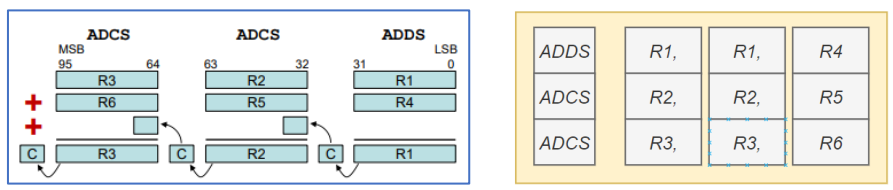
\includegraphics[width=\linewidth]{images/multiwordadd.png}

\begin{lstlisting}[language=armasm, style=basesmol]
ADDS R1, R1, R4    ; Add least significant words
ADCS R2, R2, R5    ; Add middle words with carry
ADCS R3, R3, R6    ; Add most significant words with carry
\end{lstlisting}
\end{example2}

\begin{example2}{Multi-Word Subtraction}
Subtracting 96-bit values using SBCS:

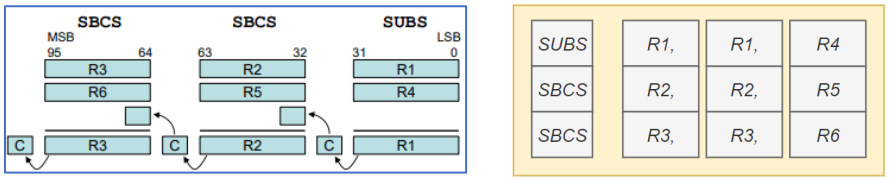
\includegraphics[width=\linewidth]{images/multiwordsub.png}

\begin{lstlisting}[language=armasm, style=basesmol]
SUBS R1, R1, R4    ; Subtract least significant words
SBCS R2, R2, R5    ; Subtract middle words with borrow
SBCS R3, R3, R6    ; Subtract most significant words with borrow
\end{lstlisting}
\end{example2}

\begin{example2}{64-bit Operations}\\
Given 64-bit variables:
\begin{lstlisting}[language=armasm, style=basesmol]
    AREA    progData, DATA, READWRITE
Long1   DCD     0      ; low word
        DCD     0      ; high word
Long2   DCD     0      ; low word
        DCD     0      ; high word
Long3   DCD     0      ; low word
        DCD     0      ; high word
\end{lstlisting}

64-bit addition:
\begin{lstlisting}[language=armasm, style=basesmol]
; Long3 = Long1 + Long2
LDR     R0, =Long1
LDM     R0!, {R1-R4}      ; Load all words
ADDS    R1, R1, R3        ; Add low words
ADCS    R2, R2, R4        ; Add high words with carry
LDR     R0, =Long3
STM     R0!, {R1, R2}     ; Store result
\end{lstlisting}

64-bit subtraction:
\begin{lstlisting}[language=armasm, style=basesmol]
; Long3 = Long2 - Long1
LDR     R0, =Long1
LDM     R0!, {R1-R4}      ; Load all words
SUBS    R3, R3, R1        ; Subtract low words
SBCS    R4, R4, R2        ; Subtract high words with borrow
LDR     R0, =Long3
STM     R0!, {R3, R4}     ; Store result
\end{lstlisting}
\end{example2}









